%Summary: Introduce idea of end to end toolflow
%Goal: Defend the idea that we can design an instrument using only a simple high level specification

%Summary: describe CASPER, PASP and reconfigurable heterogeneous setispec Goals:
%describe the existence and continued development of �blocks�
%show the ability to design reconfigurable instruments by adding a layer of abstraction to the CASPER+xgpu work

\chapter{High Level Toolflow}

%TODO
Introduction - resummarize problem solved by this work
overview of the steps in the process
include images from dissertation talk

%TODO: reword
Instrument design is often done by building the instrument from scratch.
This work extends the CASPER philosophy, demonstrating that entire instruments can be generated with minimal user input.
Rather than designing a completely different instrument for every different specification, this software package is parameterized so a change in specification only requires a recompile.

%A number of options are available but which is best?
%Need to understand how to choose the right platform(s) for each implementation
%With constant changes in technology and algorithm implementations an automatic approach is required

In this chapter, I introduce a toolflow called ORCAS or Optimal Rearrangement of Cluster-based Astronomy Signal processing .

%Describe what the tool flow should to, for whom, etc
\section{ORCAS Goals} \label{High Level Toolflow:ORCAS Goals}
ORCAS extends the CASPER philosophy discussed in Section \ref{Related Work:Radio Astronomy} by providing an end-to-end toolflow that allows the user to go from a high level description of the instrument to a low level implementation automatically. 


In order to be useful, this tool cannot rely on a single static set of blocks.

Ideal instrument design

Buy technology at the last minute

Ensure we get the best price for the performance we need

Choose hardware based on cost (\$, watts, rack space)

Low instrument development time

Assess impacts of potential optimization without implementing anything

Quickly assess performance on new or nonexistent technology

Reduce debugging time on new platforms

Support whatever hardware is currently most appropriate

%TODO: Discuss cost here. What does it mean etc...
While the x of a design has been greatly simplified by the availability of tools described in section, none of those tools help determine which type of hardware to use. %TODO add ref

Cost to include anything of value (could be dollars, could be long term use etc)

Tool supports dollars watts and user defined costs

%Goals
%Interface
%Accessible to astronomers (domain experts)
ORCAS is designed to be be accessible to both computer experts and radio astronomers, or other domain experts.
For a domain expert,  ORCAS allows the user to choose a predefined instrument type without worrying how it will ultimately map to hardware.
%Accessible computer experts
%Implementation
%Generate code for an instrument optimally mapped across a heterogeneous cluster
%Retain improvements offered by low-level optimization

The computer expert can use the tool to define a new instrument, by specifying the algorithm, and is able to provide optimization.
%TODO: fix this, I don't like it
For example, if an engineer wrote an optimized FFT algorithm, the tool will be able to incorporate that into the final optimized result.
In the end, regardless of who is using this tool, a cost-optimal mapping of the instrument gets produced. 

%TODO: Add description
\begin{figure}[ht!]
  \centering
    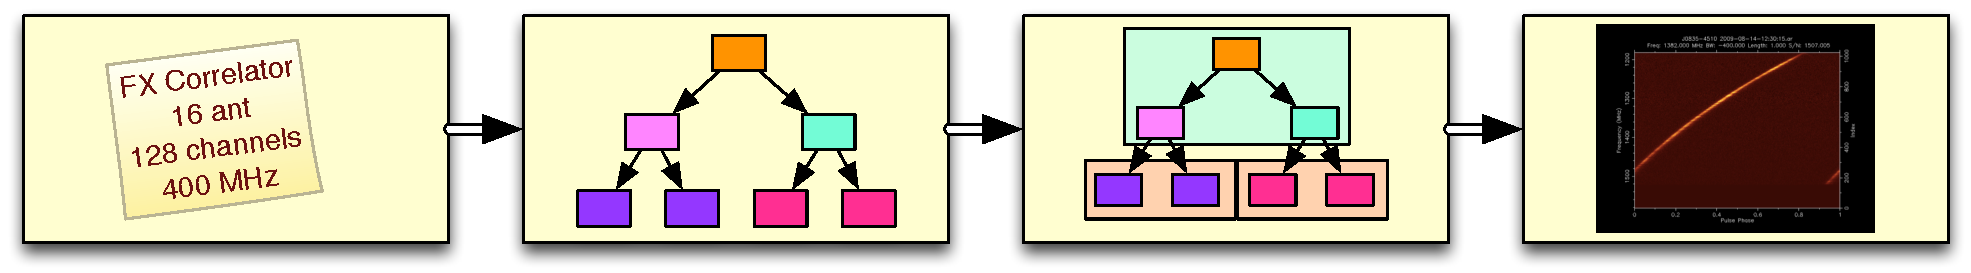
\includegraphics[width=1\textwidth]{Images/C4/toolflow_horizontal.pdf}
  \caption{The ORCAS Toolflow}
  \label{fig: C4/toolflow_horizontal.pdf}
\end{figure}

These goals are achieved through a four stage tool that allows the user to go from a high level description of an instrument to an optimized cluster design. 
Each stage of the ORCAS toolflow is represented in Figure \ref{fig: C4/toolflow_horizontal.pdf}. 
The first stage is instrument definition, which is described in Section \ref{High Level Toolflow:Instrument Definition}. 
This stage is designed to fit the needs of the domain expert. 
It allows the radio astronomer to create a predefined instrument using a handful of parameters. 
The instrument definition is converted into a dataflow model, as described in Section \ref{High Level Toolflow:Dataflow Model}. The second stage, the dataflow model is aimed at the computer expect, since it allows for a more detailed and flexible definition of the algorithm than the previous stage and provides the means to include optimized blocks.  The dataflow model represents an abstract definition of the algorithm without taking into account the eventual hardware target. The next stage, appropriately named mapping, maps the dataflow model to specific hardware. In the mapping stage, each block defined by the dataflow model gets mapped to a specific piece of hardware. This stage takes into account hardware and network limitations to produce a cost optimal mapping of the original dataflow. Finally, once each block has been mapped to a piece of hardware, the code can be stitched together into a working instrument. The rest of the chapter will describe each stage of the toolflow in more detail and explain how they are designed to meet the needs of the users they are targeting.





\section{Instrument Definition} \label{High Level Toolflow:Instrument Definition}

%TODO: Add tool name
\begin{figure}[ht!]
  \centering
    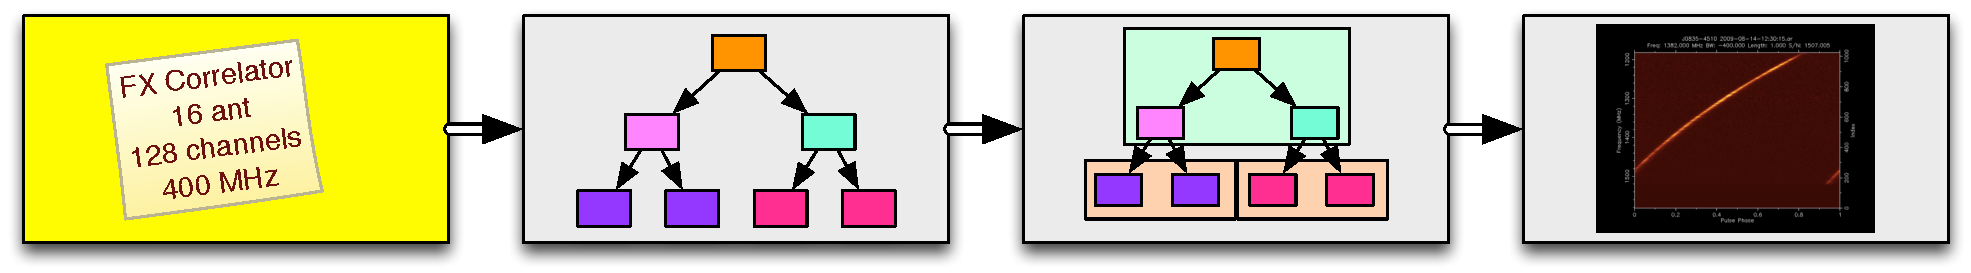
\includegraphics[width=1\textwidth]{Images/C4/toolflow_horizontal_s1.pdf}
  \caption{The ORCAS Toolflow}
  \label{fig: C4/toolflow_horizontal_s1.pdf}
\end{figure}

In the first step in the ORCAS toolflow, the user must describe the instrument using high level parameters. 
These parameters should all be relevant to the astronomer and abstract away any implementation details that do not pertain to the scientific goals. 
While it would be easy to expose many of the low level parameters at this top layer, this would force the domain expert to become a computer expert as well, exactly the scenario this tool is aiming to avoid. 


The instrument description as represented in Figure \ref{fig: C4/toolflow_horizontal_s1.pdf} fits on a small sticky note. 
The idea that the parameters should be so few that they fit on a single sticky note was the driving force behind the instrument definition. 
An instrument designer who finds that he or she needs additional control beyond what is provided by the instrument description always has the flexibility to work with the dataflow model directly, where many low level parameters are exposed. 
%TODO: why so few parameters?

%TODO: exploration
%TODO: discuss this more thoroughly
\subsection{Design space exploration}
In addition to defining a single instrument, an astronomer can use this tool to 

coarse vs fine tradeoff, ringing, algorithm

search a space of possible instruments



%Describe instrument using parameters an astronomer can understand
%Small number of predefined instrument types
%Need to input
%Instrument type (predefined patterns)
%Total Bandwidth
%Array size (n)
%Etc
%Generates a dataflow representation

%TODO: add filter parameters, ntaps, window (?)
\subsection{Supported Instruments}
%TODO: revisit this, add beamformer
Currently, the tool supports 4 instrument types: Spectrometer, High Resolution Spectrometer, Pulsar Processor, and FX Correlator, as defined in Sections \ref{Real Time Radio Astronomy Algorithms:Spectroscopy}, \ref{Real Time Radio Astronomy Algorithms:Pulsar Processing}, and \ref{Real Time Radio Astronomy Algorithms:Correlation}. 
Each instrument type has a set of parameters relevant to that instrument. 
Additional instruments or new parameters for existing instruments can be added by defining how those parameters affect the final dataflow diagram. 
This translation is described further in the next section.

\subsubsection{Spectrometer Definition}
Defining a simple spectrometer requires very few parameters. 
First, as with most instruments, the astronomer must specify the sky bandwidth the instrument must process, defined in MHz.
Then, the desired spectral resolution is defined in MHz per channel, or analogously, the number of channels that should be used to break up the bandwidth.
Finally, the integration time needs to be defined.

An additional parameter, number of antennas, can also be defined. 
This effectively describes the number of independent spectrometers that need to be created.
While this parameter does not affect the end to end processing for each antenna, knowing how many spectrometers are needed allows for more efficient use of the hardware.
The impact on the design is described further in Sections \ref{High Level Toolflow:Dataflow Model} and \ref{High Level Toolflow:Mapping} and the efficiency afforded by this parameter is explored in Chapter \ref{Analysis}

\subsubsection{High Resolution Spectrometer Definition}
The main difference between a spectrometer and a high resolution spectrometer is the need for two stages of channelization rather than just one. 
The sky bandwidth, integration time, and number of antennas are defined in the same way as the previous spectrometer. 

The spectral resolution is defined differently, because both the coarse and fine resolutions need to be defined. 
The coarse resolution defines how many channels the whole sky bandwidth should be broken up into initially.
The fine resolution defines how many channels each coarse channel is broken into.
Both can be described in MHz per channel or by just giving the number of channels required to break up the band.

%TODO: Ask Jonathon about this
\subsubsection{Pulsar Processor Definition}
Bandwidth

Number of channels for each part

Integration time

nant

\subsubsection{FX Correlator Definition}
Bandwidth

nant

number of channels

integration time








\section{Dataflow Model} \label{High Level Toolflow:Dataflow Model}
%TODO: Add tool name
\begin{figure}[ht!]
  \centering
    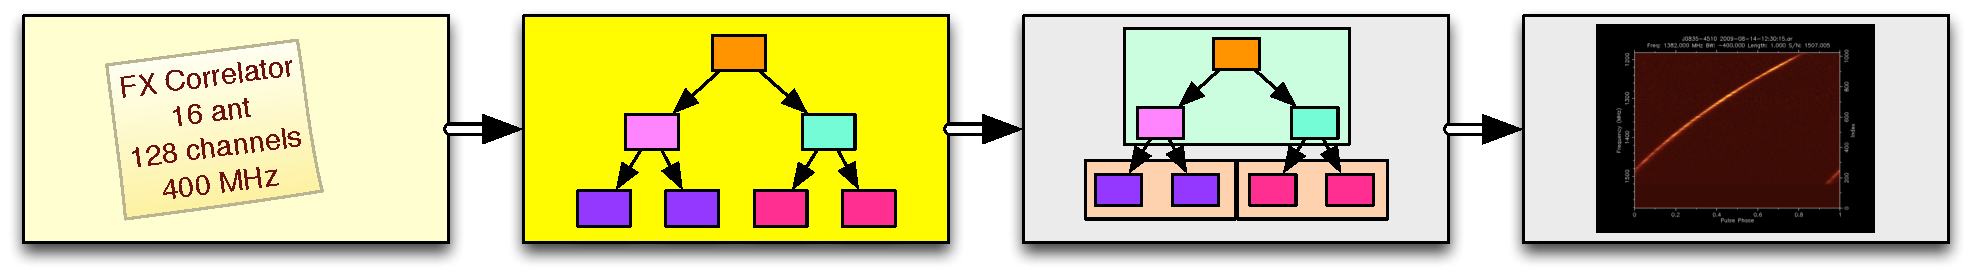
\includegraphics[width=1\textwidth]{Images/C4/toolflow_horizontal_s2.pdf}
  \caption{TODO Toolflow}
  \label{fig: C4/toolflow_horizontal_s2.pdf}
\end{figure}

%\subsection{Overview}

%Dataflow representation of instrument
%Define input/output connections
%Define input/output bandwidth
%Generates a series of blocks configured to talk to each other

\subsection{Computational Blocks}
%Collection of blocks necessary to solve most problems
%Can be parameterized
%Include a method to assess performance on each (supported) platform
%Performance model
%Benchmark
%Unit tests
%Uniform interconnect model
%Optimization: remove interconnect overhead for cores running on the same hardware

%Not certain this belongs here, possibly should go with the models?
%Before mapping, need to determine which blocks can be mapped to which platforms
%Synthesize/compile existing implementations to determine which platforms can support the spec
%Sanity check bandwidth requirements
%Test for acceptable noise tolerance in different implementations
%Known signals
%Test against arbitrary precision (exact) floating point implementation

%Optimization already exists
\cite{Govindaraju:2008vx} %replace with more recent fft alt
\cite{Kestur:2010tn}


\subsection{Connection Types}

Suppose we know we have 2 types of blocks: $A$, and $B$. 
Blocks of type $A$ must send their output to blocks of type $B$.
Now, we need to understand how blocks of type $A$ send data to blocks of type $B$.
This could happen in 2 ways, `one-to-one' and `all-to-all'. 

%TODO: fix references
\begin{figure}
  \centering
    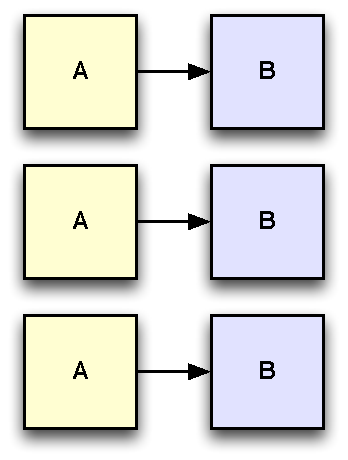
\includegraphics[width=0.45\textwidth]{Images/C5/one-to-one.pdf}
    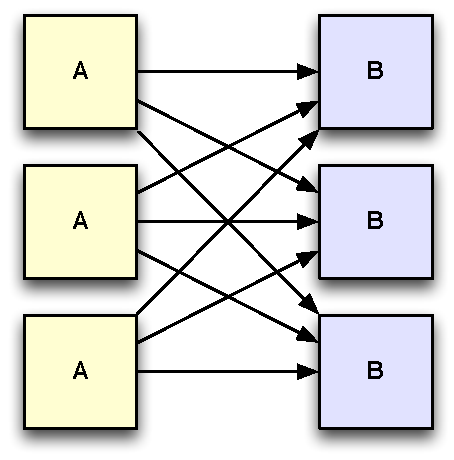
\includegraphics[width=0.45\textwidth]{Images/C5/all-to-all.pdf}
  \caption{TODO}
  \label{fig:C4/one-to-one.pdf}
\end{figure}

A `one-to-one' connection is where every block of type $A$ communicates with exactly one block of type $B$, as shown in Figure \ref{fig:C4/one-to-one.pdf}. 
With this type of connection, the number of blocks of type $A$ must be equal to the number of blocks of type $B$.
The F-engines in a FX correlator are a good example of this type of connection. 
The correlator has an F-engine for each antenna, each containing the same blocks linked in the same way. 
Within an F-engine, a PFB\_FIR filter must communicate with a single FFT.
In general, every PFB\_FIR within an F-engine, blocktype `A' must communicate with exactly one FFT, blocktype `B'. 
      



An `all-to-all' connection occurs when every block of type $A$ must send some data to ever block of type $B$. 
Figure \ref{fig:C4/all-to-all.pdf} shows what an all-to-all connection between 3 blocks of type $A$, and 3 blocks of type $B$ will look like. 
In this case, every block of type $A$ must send some data to every block of type $B$. 
For example, the type of connection between the per-antenna FFTs and the per-channel X-engines in an FX correlator would be `all-to-all'. 
Each X-engine needs a small amount of data from every F-engine to compute the cross-correlations from a single channel. 
In the `all-to-all' case, there is no reason for the number of sending nodes needs to be the same as the number of receiving nodes. 
%The n's do not get introduced until the ILP is defined
%This means that $n_{i,A}$ and $n_{i,B}$ do not have to be equal, and as long as the data can be distributed appropriately, there is no enforced relationship between the two variables. 




%TODO: make this an a,b figure
\begin{figure}
  \centering
    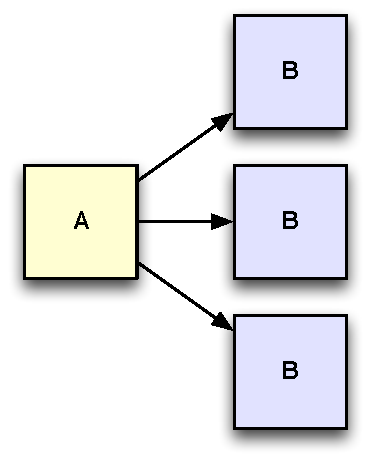
\includegraphics[width=0.4\textwidth]{Images/C5/one-to-all.pdf}
    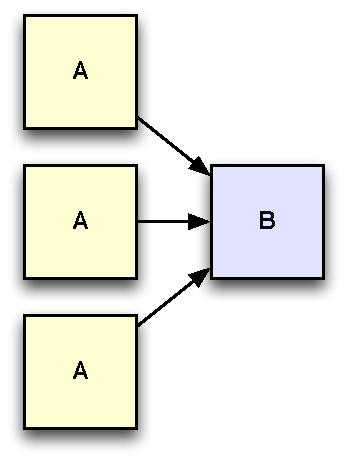
\includegraphics[width=0.4\textwidth]{Images/C5/all-to-one.pdf}
  \caption{TODO}
  \label{fig: C4/one-to-all_vs_all-to-one}
\end{figure}



It might seem like there are two more possible types of connection, `one-to-all' and `all-to-one' .
A data flow with a `one-to-all' connection, shown in Figure x %TODO: fix reference, image
would have exactly one block of type $A$ that needs to send data to many blocks of type $B$. 
This is exemplified in the dataflow for a high-resolution spectrometer.
The coarse channelization is done in a single FFT block, which then needs to send the data to many other FFTs to do the fine channelization. 
The `all-to-one' connection shown in Figure x %TODO: fix ref
is there reverse of the `one-to-all' case. 
In this type of connection, there are many blocks of type $A$ and they all need to send data to a single instance of a block of type $B$. 
An example of this arises when some processing is done in a distributed manner but the instrument needs to record the final result in a central place. 
The $A$ blocks are responsible for the distributed processing, and then the $B$ block needs to collect the results and combine them.
%TODO: discuss scatter-gather?

It turns out, these are both special instances of the `all-to-all' connection. 
The `one-to-all' connection is simply an `all-to-all' where the number of $A$ blocks is fixed at 1.
Similarly, the `all-to-one' connection is also an `all-to-all' where the number of $B$ blocks is fixed at 1.
Because of this, there is no need to include or support these cases as unique connection types. 


While it may seem like additional link types exist like `all-to-some' or `one-to-some', this turns out to be impossible. 
Either a block of type $A$ cannot send its data to only some blocks of type $B$ because of the way blocktypes are defined.
Any block of the same type should be interchangeable with another block of the same type.
In an `all-to-some' connection, blocks of type $A$ would need to send data to $B_1$ but not send data to $B_2$.
But that connection patterns implies that the blocks $B_1$ and $B_2$ are \emph{not} interchangeable and therefore cannot have the same blocktype.


%TODO: This isn't implemented in the ILP
%TODO: Add correlator beamformer example. 
This does not preclude asymmetrical designs. 
Instead, asymmetry is supported by allowing blocks to define a list of blocktypes they must send data to or receive data from. 
The connection between any two blocktypes still must be described as above.

\subsection{Translating Instrument Definitions to Dataflow Diagrams}
% Describe data flow for each instrument we are interested in implementing
Now that we have a method for describing a general dataflow, we will describe how each type of instrument definition described in the previous section is converted to a dataflow. 


\subsubsection{Spectrometer}

\begin{figure}[ht!]
  \centering
    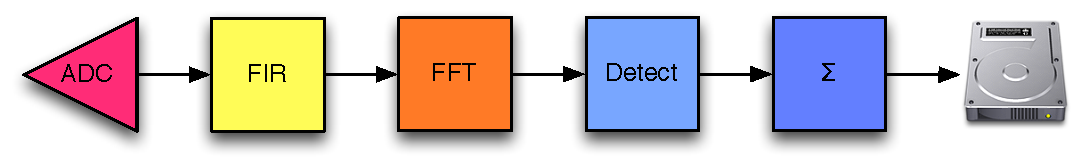
\includegraphics[width=1\textwidth]{Images/C4/spectrometer_dataflow.pdf}
  \caption[General Spectrometer Dataflow Model]{General Spectrometer Dataflow Model.
  \textit{
  A general dataflow model for a single antenna spectrometer. 
  This model can be applied to any spectrometer, as the spectrometer parameters do not affect how many computational blocks are required or the interconnect layout. 
  %TODO: This is questionable, ask dan
  The data is fed in by an ADC and filtered using an FIR to improve the response of the FFT.
  The filtered data is then channelized by an FFT, accumulated in the block labeled $\Sigma$ and recorded to disk.
  }}
  \label{fig: C4/spectrometer_dataflow.pdf}
\end{figure}

The spectrometer instrument definition generates a very simple dataflow. 
Figure \ref{fig: C4/spectrometer_dataflow.pdf} shows the general dataflow model for a spectrometer. 
The ADC feeds data into a FIR filter. 
Then the filtered signal is transformed into channels in the FFT and those channels are accumulated and saved to disk. Regardless of the parameters the astronomer chooses, the dataflow will be the same. 

The parameters for each block come directly from the instrument definition. 
The FIR parameters come from the number of FIR taps and window shape, the FFT is simply defined by the FFT length parameter and the accumulator also is parameterized by the FFT length as well as the integration time. 

%Multiple antennas?

\subsubsection{High Resolution Spectrometer}

\begin{figure}[ht!]
  \centering
    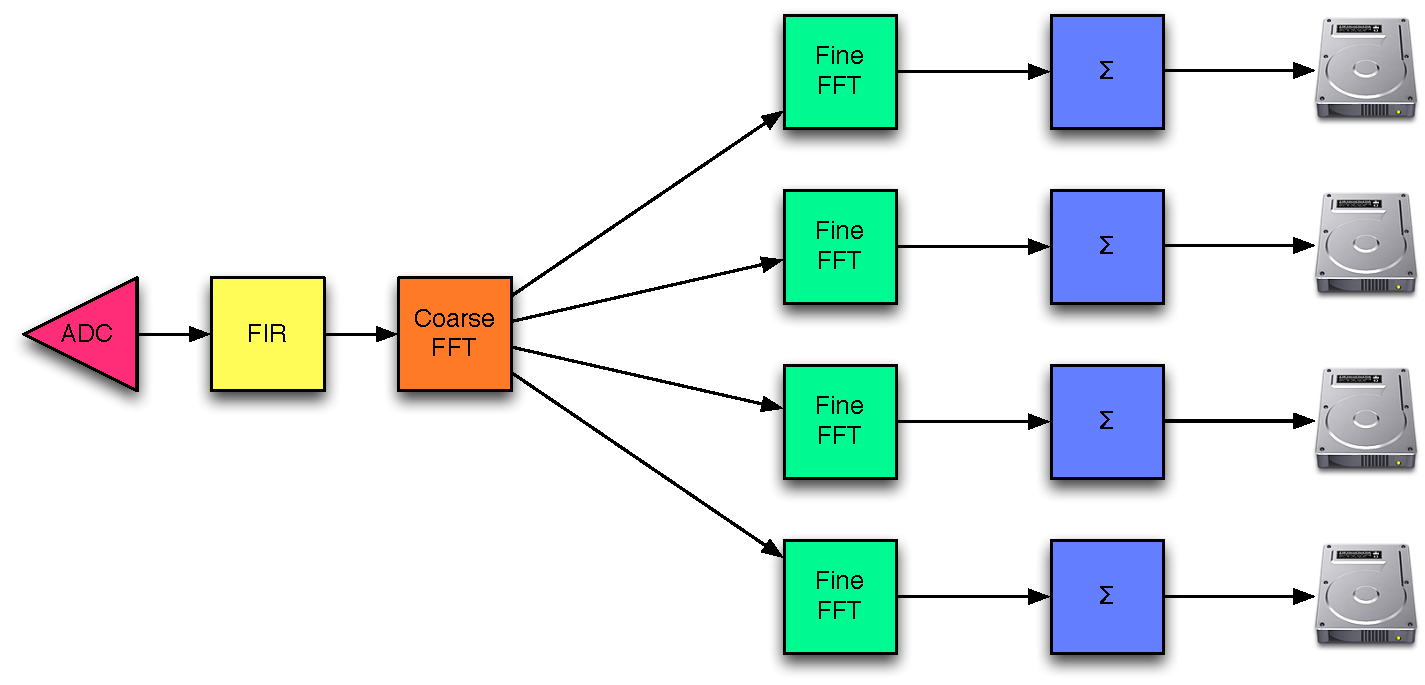
\includegraphics[width=1\textwidth]{Images/C4/hires_spectrometer_dataflow.pdf}
  \caption[Example High Resolution Spectrometer Dataflow Model]{Example High Resolution Spectrometer Dataflow Model
  \textit{
  This figure shows an example dataflow for a high resolution spectrometer with 4 coarse FFT channels.
  Like the previous spectrometer, the data comes in through an ADC, is filtered and then channelized using a coarse FFT.
  Then, to achieve a higher resolution, each coarse channel is divided into sub-channels using the 4 fine FFT blocks in the dataflow. 
  }}

  \label{fig: C4/hires_spectrometer_dataflow.pdf}
\end{figure}

The high resolution spectrometer dataflow does depend on the parameters specified in the instrument description. 
An example dataflow is shown in Figure \ref{fig: C4/hires_spectrometer_dataflow.pdf}. 
The first three blocks in the dataflow are exactly the same as the Spectrometer dataflow described in the previous section. 
An ADC feeds data into a FIR filter followed by an FFT. 
After the FFT, the algorithm is modified to accommodate the higher resolution required. 
The first FFT divides the band into a number of coarse channels and then each coarse channel must be further divided into a number of fine channels. 
The coarse FFT must feed its data to a separate fine FFT for each coarse channel, so the number of fine FFTs in the dataflow diagram will vary based on the number of coarse channels.
At this point, each coarse channel is processed in an independent pipeline the finely channelized data is accumulated and recorded to disk. 
The example in Figure \ref{fig: C4/hires_spectrometer_dataflow.pdf} shows a spectrometer that divides the data into 4 coarse channels.


%TODO Finish: graphic for F/X engine, name sub channelization step (S?)

%Multiple antennas?

\subsubsection{FX Correlator}

The FX dataflow model is based on the algorithm architecture for the CASPER correlator described in Section \ref{Related Work:Radio Astronomy}. The processing model is described by replicating 2 basic pipelines, called an F-Engine and an X-Engine. An F-Engine, pictured in Figure \ref{fig: C4/fx_f_engine.pdf} is responsible for channelizing the data from a single antenna. It takes in data from an ADC, and channelizes the data using a FIR and FFT to create a polyphase filter bank. 

\begin{wrapfigure}{L}{0.50\textwidth}
  \centering
    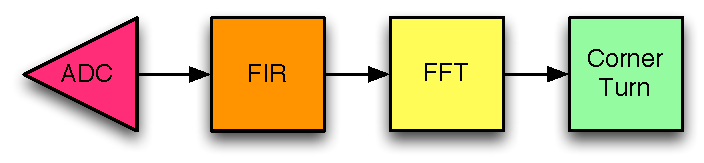
\includegraphics[width=0.48\textwidth]{Images/C4/fx_f_engine.pdf}
  \caption{FX Correlator F-Engine Model}
  \label{fig: C4/fx_f_engine.pdf}
\end{wrapfigure}

\begin{wrapfigure}{R}{0.50\textwidth}
  \centering
    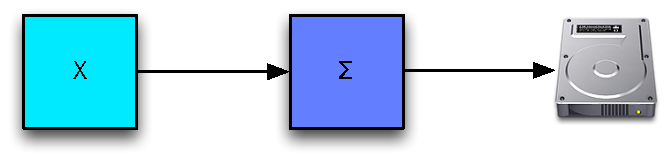
\includegraphics[width=0.48\textwidth]{Images/C4/fx_x_engine.pdf}
  \caption{FX Correlator X-Engine Model}
  \label{fig: C4/fx_x_engine.pdf}
\end{wrapfigure}


\begin{figure}[ht!]
  \centering
    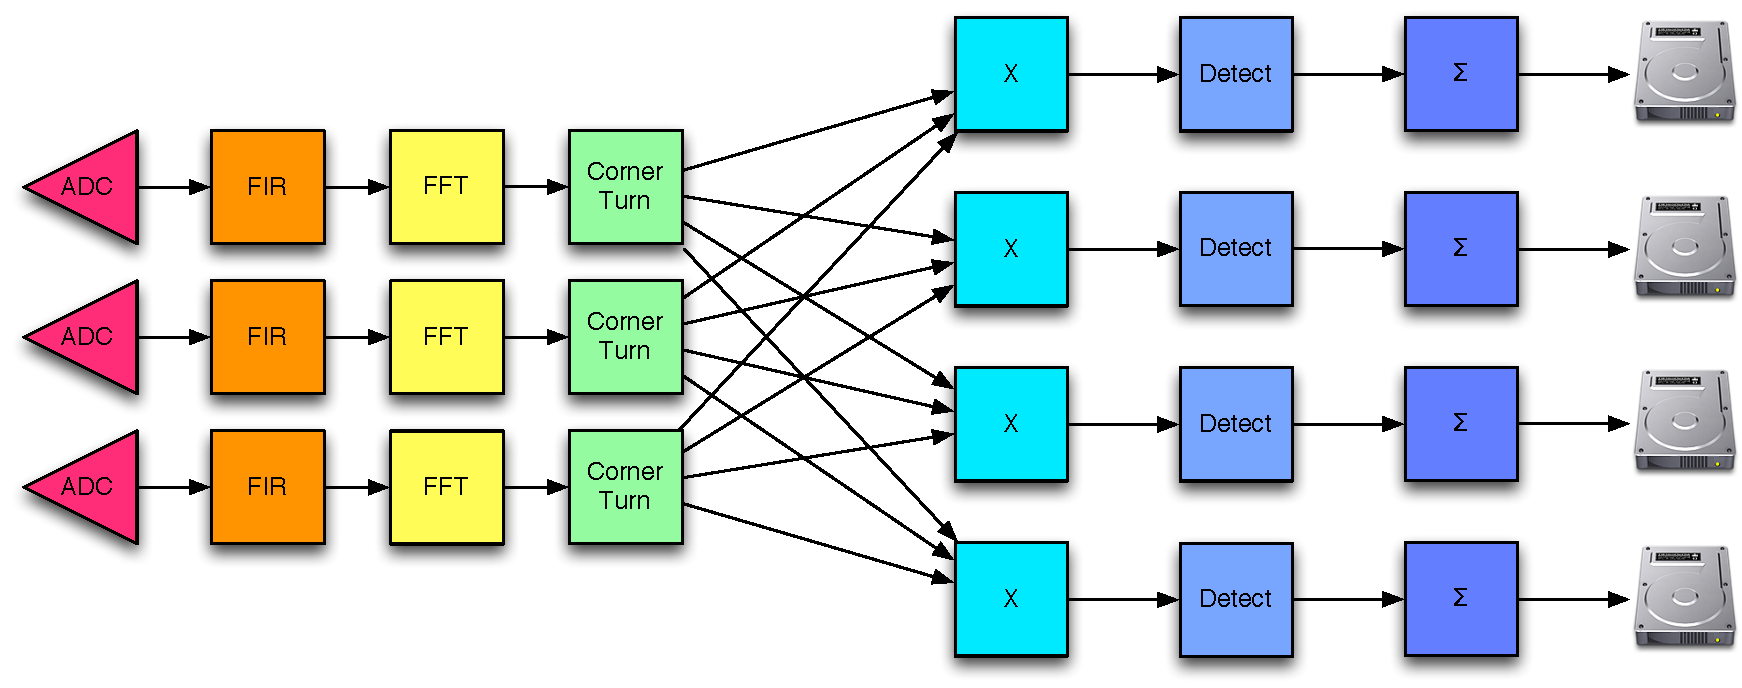
\includegraphics[width=1\textwidth]{Images/C4/fx_dataflow.pdf}
  \caption{Example FX Correlator Dataflow Model}
  \label{fig: C4/fx_dataflow.pdf}
\end{figure}

The dataflow for an FX correlator will vary quite a bit based on the input parameters. Figure \ref{fig: C4/fx_dataflow.pdf} shows an example 3 antenna 4 channel. 

\section{Mapping}  \label{High Level Toolflow:Mapping}
%TODO: Add tool name
\begin{figure}[ht!]
  \centering
    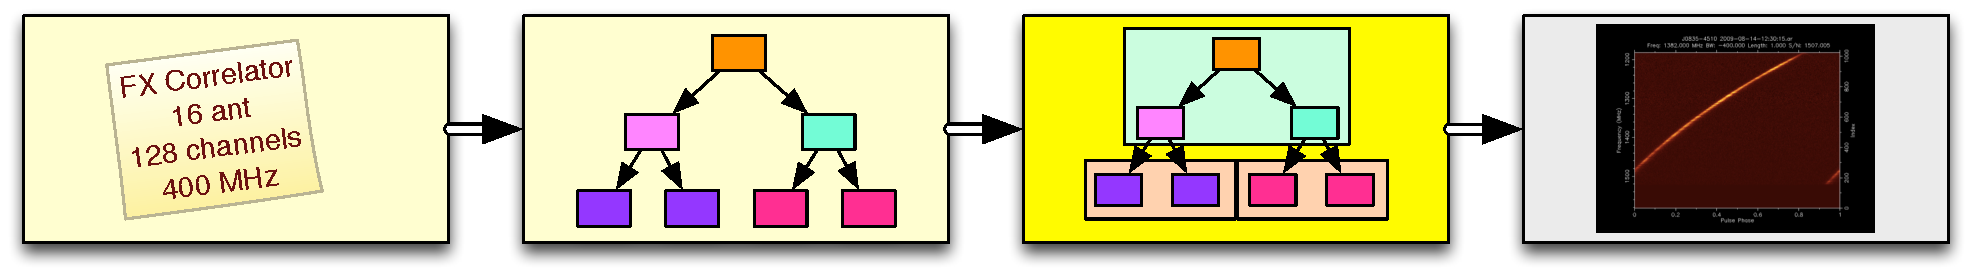
\includegraphics[width=1\textwidth]{Images/C4/toolflow_horizontal_s3.pdf}
  \caption[ORCAS Toolflow]{ORCAS Toolflow Mapping}
  \label{fig: C4/toolflow_horizontal_s3.pdf}
\end{figure}

Once the dataflow and the computational blocks are defined, ORCAS must determine how to place each computational block into hardware. 
In the mapping stage, ORCAS determines what type of hardware should be used for each block, while minimizing the total cost of the hardware (in dollars, watts, or another used-defined metric).
Figure \ref{fig: C4/toolflow_horizontal_s3.pdf} highlights the mapping phase of the toolflow. 

At this point, the computational blocks and dataflow can no longer be viewed as abstract algorithms. 
Each computational block must be paired with a performance model for each supported platform that shows the resource utilization and bandwidth requirements for that block. 
Using the performance model, the tool is able to test a number of hardware mappings and ensure that none of the available hardware or bandwidth resources are overmapped.

The optimal mapping is determined using an Integer Linear Program or ILP. 
The resources, such as memory, logic and CPU time, and bandwidth constraints are translated directly into ILP constraints.
Theseconstraints are used to determine a valid mapping, for example total bandwidth mapped to a link must be less than total link bandwidth.
The variables represent the design decisions, determining where each block should be implemented.
And finally, the cost function simply totals up the costs associated with each piece of hardware used.

%TODO: rewrite with references
A ILP was chosen because it has a number of positive features.
Unlike a randomized algorithm such as simulated annealing, the results from a ILP are repeatable.
While there might be multiple solutions with the same cost, each time the same ILP is run, it is guaranteed to find one of the solutions of optimal cost. 
The ILP representation also makes it easy for the user to guide the algorithm. 
Since the design choices are represented by variables, they can also be restricted by adding additional constraints to those variables.
This representation also makes it easy to build out an existing cluster, by allowing a limited amount of zero-cost hardware.

Unfortunately, the advantages of the ILP come with a high cost, namely that an ILP is NP-Hard to solve optimally.
%TODO: ref
Current ILP benchmarks are able to solve problems with a hundred thousand variables in a few hours, but beyond that size the problems become infeasible.
%TODO: add an ex solver
To make matters worse, the ILP runtime is very sensitive to the solver being used and the problem structure.

Because the runtime for the ORCAS mapper needs to be within a few hours, we use a number of techniques to reduce the ILP runtime.
%TODO: add more info here
First, the easiest way to reduce the runtime without changing the ILP is to change the solver. 
There is a huge amount of variance in runtimes between different solvers and simply switching out the backend solver might cause a previously infeasible problem to become solvable.
When that doesn't improve the runtime enough, it becomes necessary to modify the ILP.
One way to do this is by reducing the number of variables it needs to solve for.
Many of the radio astronomy instruments are very symmetric, so it is reasonable to assume that the optimal mapping would be symmetric as well.
The symmetry can be preserved by forcing every block of a certain type to be implemented in the same kind of hardware, drastically reducing the number of decisions that the ILP needs to make.
The ILP can also be modified to ensure that there is a single, unique optimal solution.
When designs are very symmetric, the ILP will often find an optimal solution quickly but, because it is not unique, the ILP must spend a lot of time convincing itself that the solution is, in fact, optimal.
Additional constraints can be added to ensure that only one of those solutions is valid, greatly reducing the amount of time it takes to verify optimality.

Chapter \ref{chap:Algorithm Partitioning} goes into more detail on how the performance models are used as well as how the ILP is specified and optimized to achieve a feasible runtime. 

\subsection{Mapped Dataflow Representation}

Figure \ref{fig: C4/fx_mapped.pdf} shows two example mappings for the FX Correlator dataflow shown in Figure \ref{fig: C4/fx_dataflow.pdf}.


\begin{figure}[ht!]
  \centering
    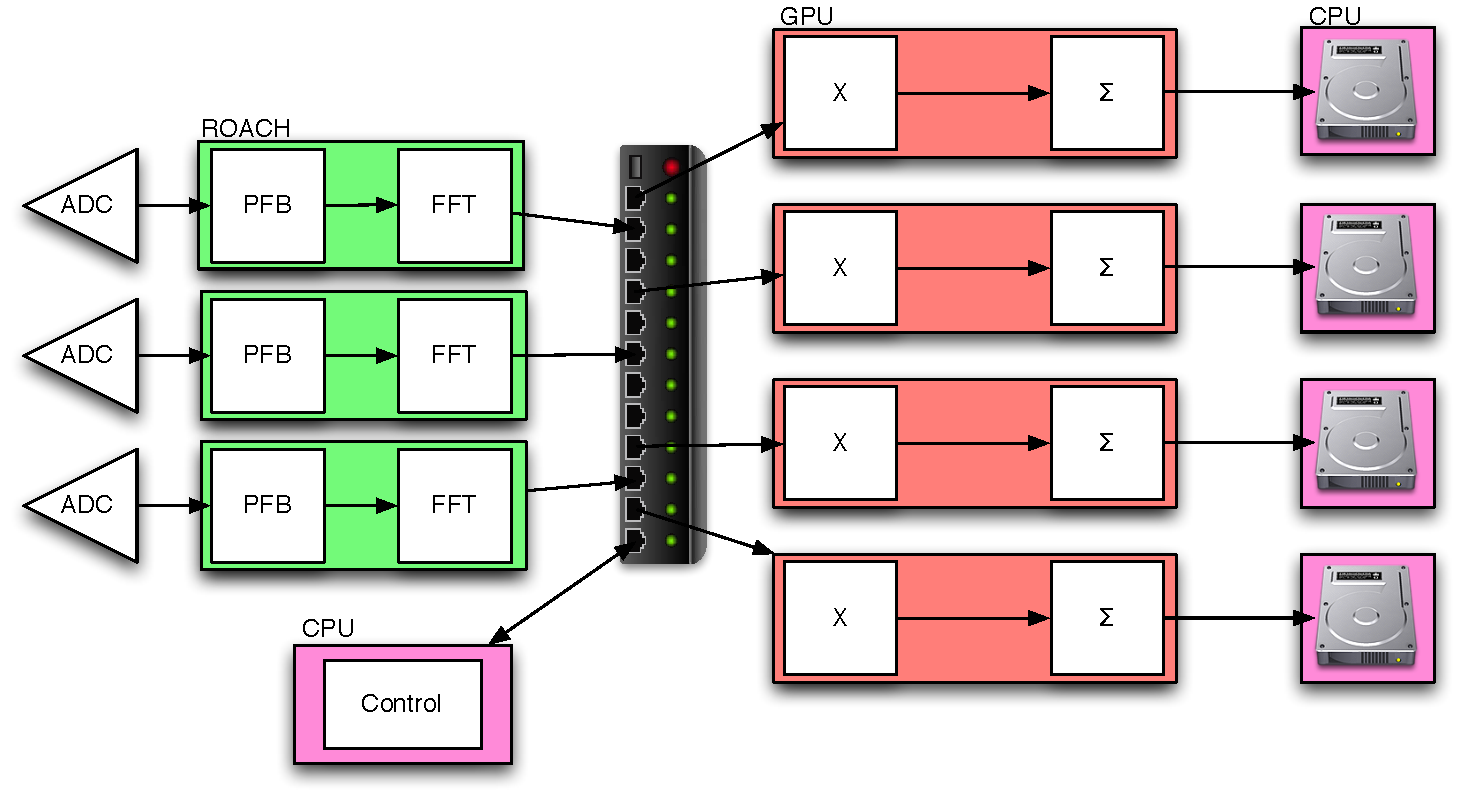
\includegraphics[width=\textwidth]{Images/C4/fx_mapped.pdf}
    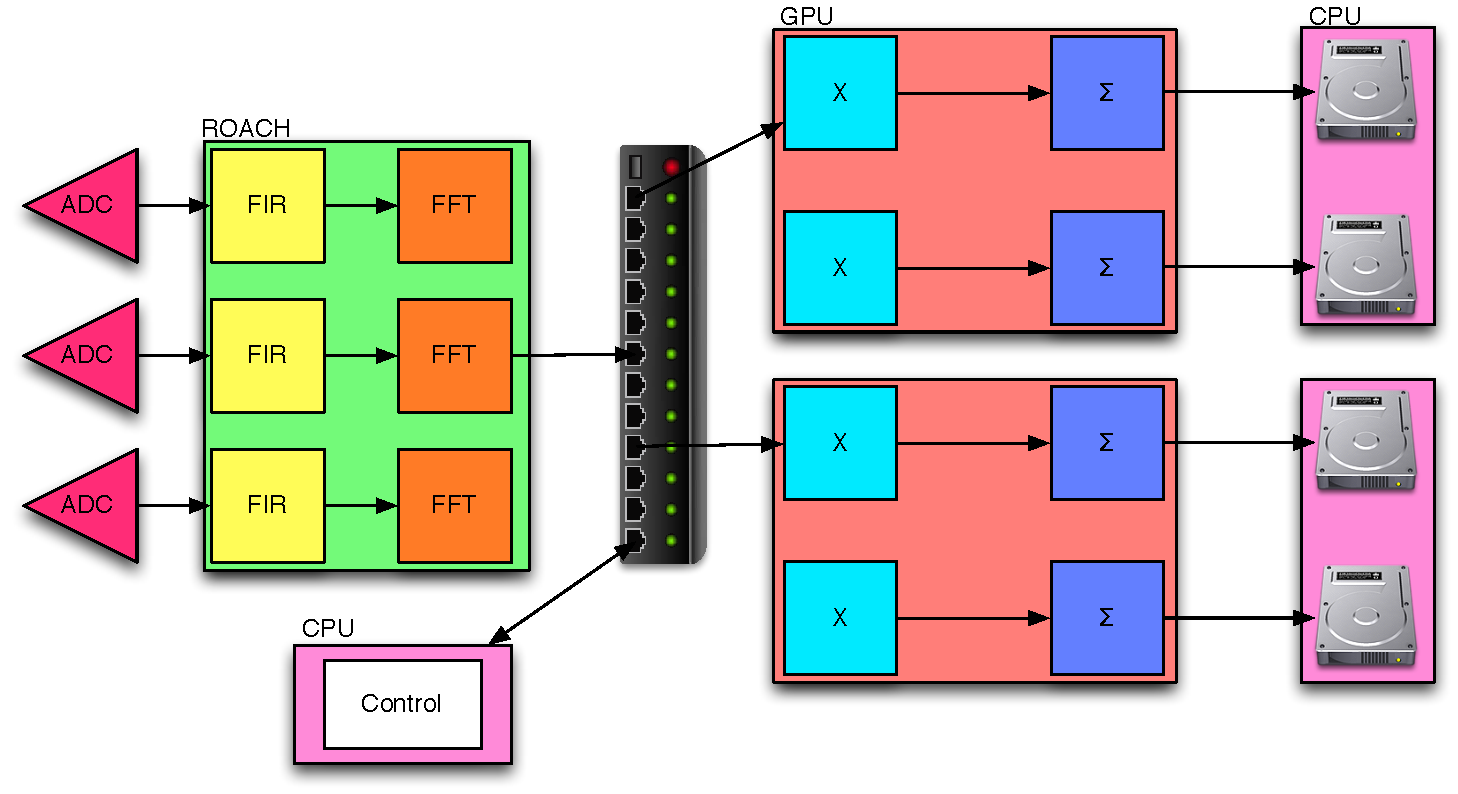
\includegraphics[width=\textwidth]{Images/C4/fx_mapped_alt.pdf}
  \caption{Two potential mappings for the FX Correlator}
  \label{fig: C4/fx_mapped.pdf}
\end{figure}






%TODO: think hard about this, we're not actually going to do this and it's optional
%This could be a good place to describe PASP, this is doable, we've shown it's possible
%Don't actually want to implement the entire thing but show feasibility
\section{Code Generation}
%TODO: edit description
\begin{figure}[ht!]
  \centering
    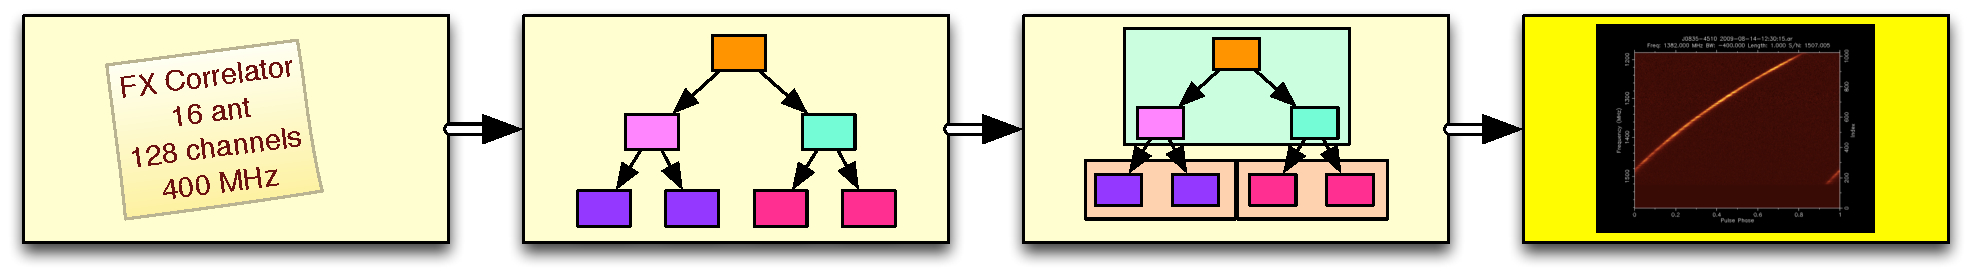
\includegraphics[width=1\textwidth]{Images/C4/toolflow_horizontal_s4.pdf}
  \caption{ORCAS Toolflow}
  \label{fig: C4/toolflow_horizontal_s4.pdf}
\end{figure}

%Use casper blocks, libraries, etc to do this
%Show that it's possible to stitch them together

%Use a mapped dataflow to stitch together blocks
%To generate code the blocks must have an implementation for the target platform (not necessary for mapping)
%Include an automatic test suite for each platform
%Block communication is standardized so they can be connected in arbitrary ways
\subsection{Packetized Astronomy Signal Processor}

%TODO
\cite{McMahon:2008tk}
\cite{Filiba:2011wl}

This instrument has a wide variety of potential applications due to the flexibility of the server software. 
In this section, we describe a few specific applications than can make use of this package.

In the search for extraterrestrial intelligence (SETI), the ability to keep up with changes in technology allows searching instrumentation to stay on the leading edge of sensitivity. 
SETI aims to process the maximum bandwidth possible with very high resolution spectroscopy.
This instrument allows SETI projects to easily keep up with improvements on the telescope and increasing computational power.
An increase in detector bandwidth, improving the breadth of the search, can be processed simply recompiling the FPGA design and distributing the extra subbands to new servers. 
As computation improves, the instrument can be reconfigured to send more bandwidth to each computer, reducing the required cluster size, or improve the resolution of the instrument by doing a larger FFT on the server.

This design also has applications in pulsar science. 
The fast channelization on the FPGA with no data reduction makes it an ideal pulsar spectrometer, since no information is lost before sending the data to the servers.
GPUs provide a good platform for pulsar processing algorithms such as coherent dedispersion \cite{Ransom:2009wz}, which can easily be used as the processing function for the server software distributed in our package. 
Similar to SETI instruments, pulsar instruments designed using this package can also keep up with improvements in technology with a simple recompile.

Figure \ref{fig: pasp_fpga_arch} gives an overview of the dataflow through the FPGA.
The FPGA interfaces to a single ADC board that simultaneously digitizes 2 signals. 
Each signal can be sampled at a maximum rate of 1Msps.
The samples are sent into a polyphase filter bank (PFB), consisting of an FIR filter and an FFT, which breaks up the entire bandwidth sampled by the ADC into smaller subbands.
After dividing up the subbands, each band is rescaled. 
This step allows us to compensate for the shape of the analog filter feeding data into the ADC. 
After rescaling, the FPGA forms packets where each packet contains data from a single subband. %TODO fix
The packets are sent out over CX4 ports to a 10 gigabit Ethernet switch.

\begin{figure}[ht!]
  \centering
    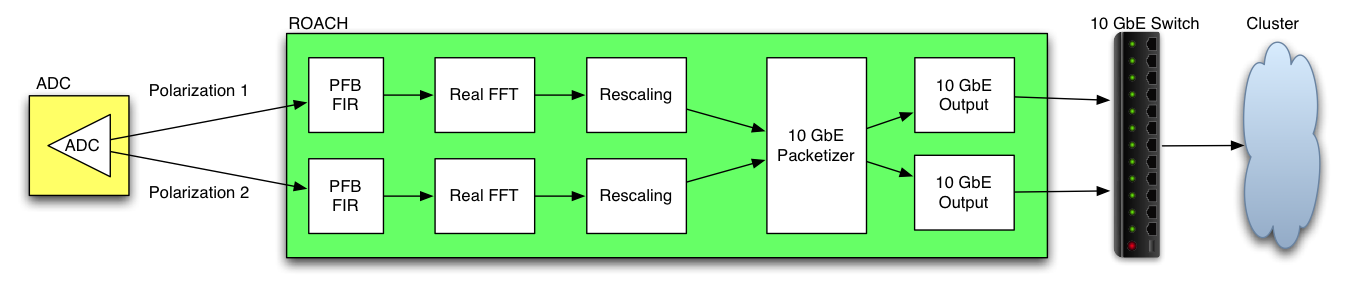
\includegraphics[width=1\textwidth]{Images/C4/pasp_fpga_arch.png}
  \caption{PASP Dataflow}
  \label{fig: pasp_fpga_arch}
\end{figure}

PASP uses a PFB to split up the subbands. Figure \ref{fig: fft_vs_pfb_response} shows a comparison between the FFT and PFB response. 
The FFT response (on the left) has a lot of spectral leakage while the PFB (on the right) has a much sharper filter shape and a better frequency response. 
The superior frequency response led us to use a PFB rather than an FFT to extract subbands, despite the additional FPGA resources required by the FIR filter before the FFT.

\begin{figure}[ht!]
  \centering
    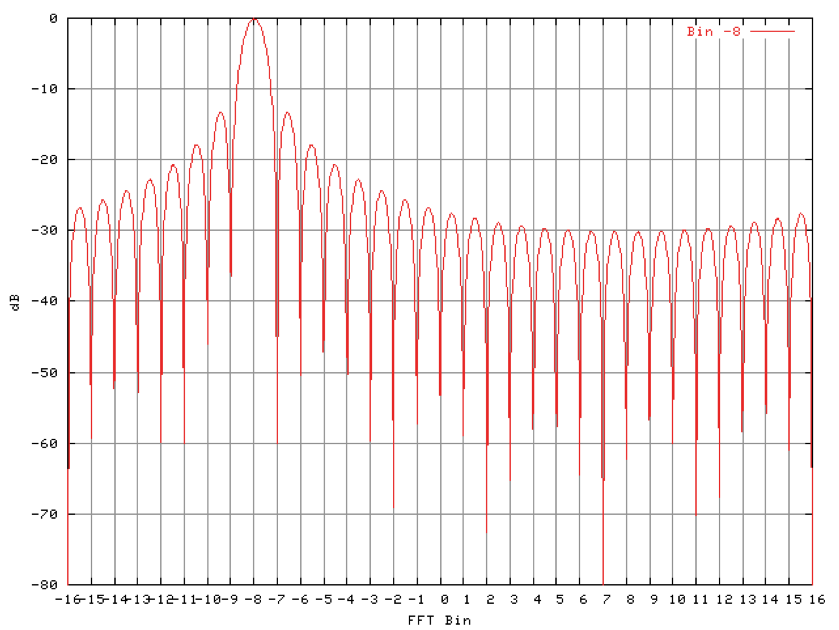
\includegraphics[width=0.48\textwidth]{Images/C4/fft_response.png}
    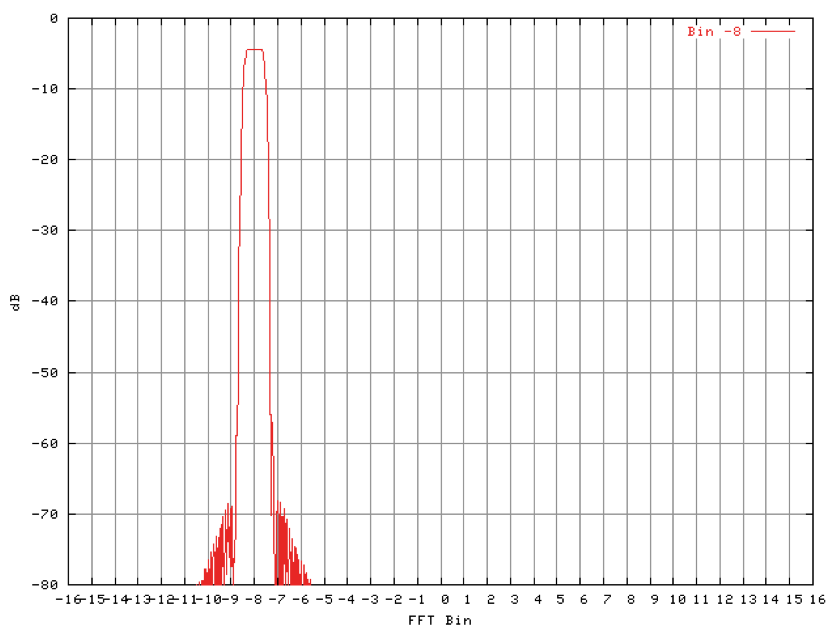
\includegraphics[width=0.48\textwidth]{Images/C4/pfb_response.png}
  \caption{A comparison of FFT and PFB response}
  \label{fig: fft_vs_pfb_response}
\end{figure}

PASP is designed for flexibility. 
Building on the CASPER goal to automate the design of commonly used signal processing elements such as FFTs and digital downconverters, PASP automatically designs an entire FPGA instrument using only a few parameters.
The user can input the desired number of subbands, CPU/GPU cluster size, and packet size and a new design is automatically generated in Simulink.  

\subsection{Heterogeneous Radio SETI Spectrometer}

\begin{figure}[ht!]
  \centering
    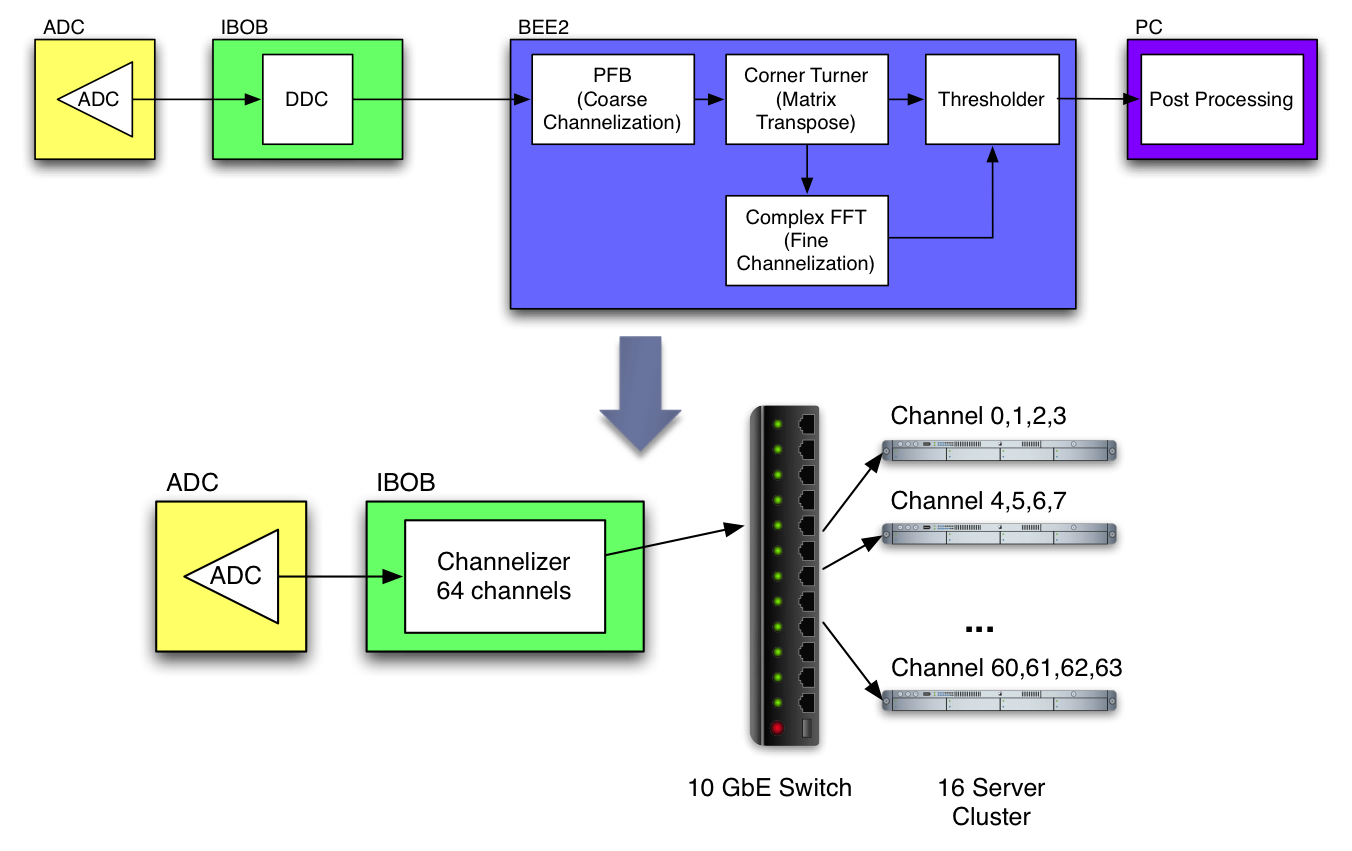
\includegraphics[width=\textwidth]{Images/C4/serendip_vv_to_hrss.png}
  \caption{TODO}
  \label{fig: C4/serendip_vv_to_hrss.png}
\end{figure}


We have developed a software package to automatically generate spectrometers with minimal user input.

We have automated this design, creating a parameterized spectrometer that only requires a recompile to implement a change in specification.
This spectrometer combines FPGAs and GPUs, doing coarse channelization on the FPGA and sending each subband to the GPUs for further processing.
The server software is designed for flexibility, allowing astronomers to easily modify the processing algorithm run on the GPU and customize the instrument to fit their science goals.

The software package includes an FPGA design and server software to do spectroscopy, as well as server benchmarks used to determine an optimal instrument configuration.
%The benchmarks measure maximum amount of data the servers can process, determining the optimal configuration for the instrument.
Both the FPGA and server software are parameterized, allowing for rapid deployment of a working spectrometer that is configured to take full advantage of available computing resources.
%Our general purpose approach allows for the rapid development of new instruments.
We implement the instrument on a heterogeneous cluster consisting of both FPGAs and GPUs to take advantage of the benefits provided by both platforms.
FPGAs provide high bandwidth processing but can be cumbersome to program.
GPUs can't handle the same bandwidths as FPGAs but they are easier to program. 
The CUDA language, for example, is a C-like language that can be used to develop software for many GPUs.
The high level parameters in this package allow us to use FPGAs while abstracting away implementation details specific to the FPGA.
To give the user control over their data processing algorithm, an application specific GPU program can be written and easily interfaced with the existing receive software in the package.

%TODO fix this
\begin{figure}[ht!]
  \centering
    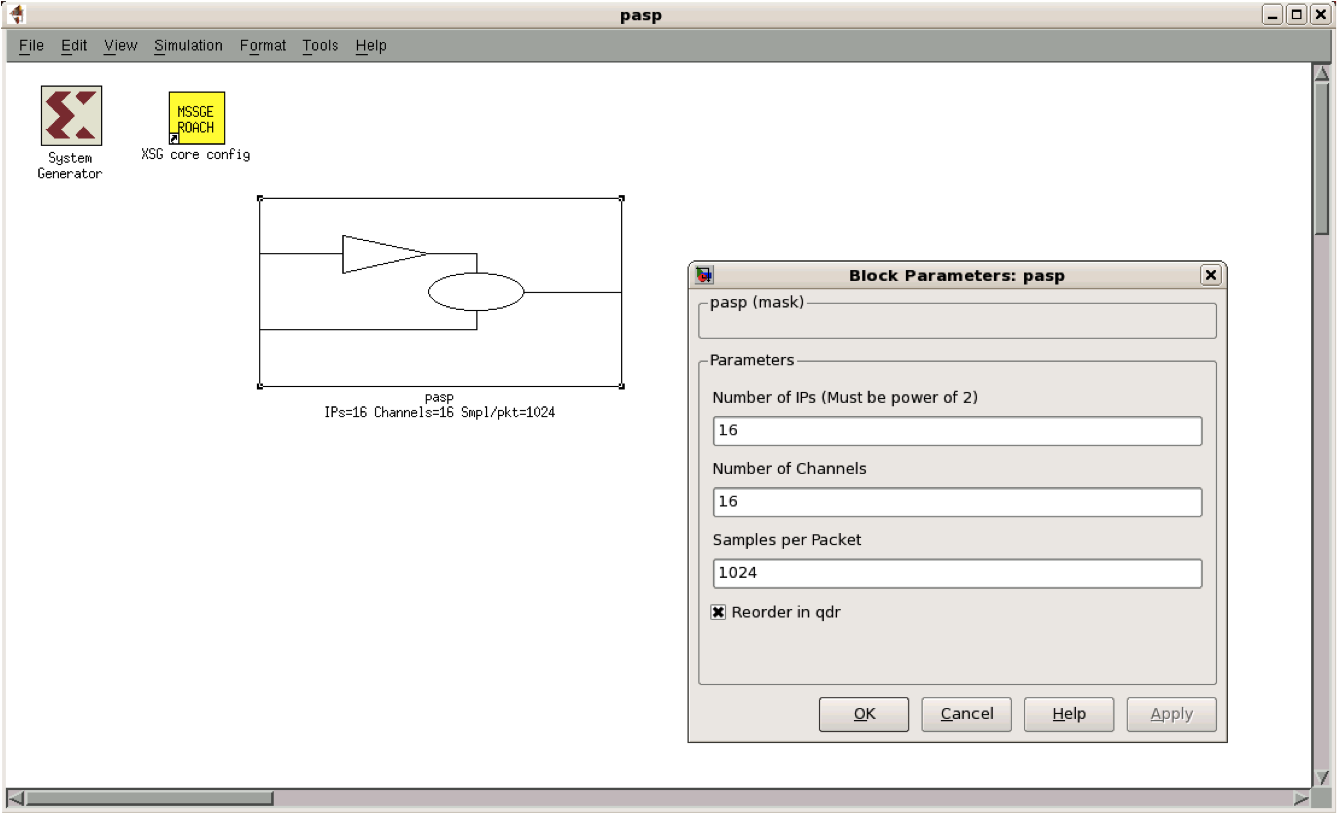
\includegraphics[width=0.49\textwidth]{Images/C4/pasp_high_level_interface.png}
  \caption{TODO}
  \label{fig: C4/pasp_high_level_interface.png}
\end{figure}

\begin{figure}[ht!]
  \centering
    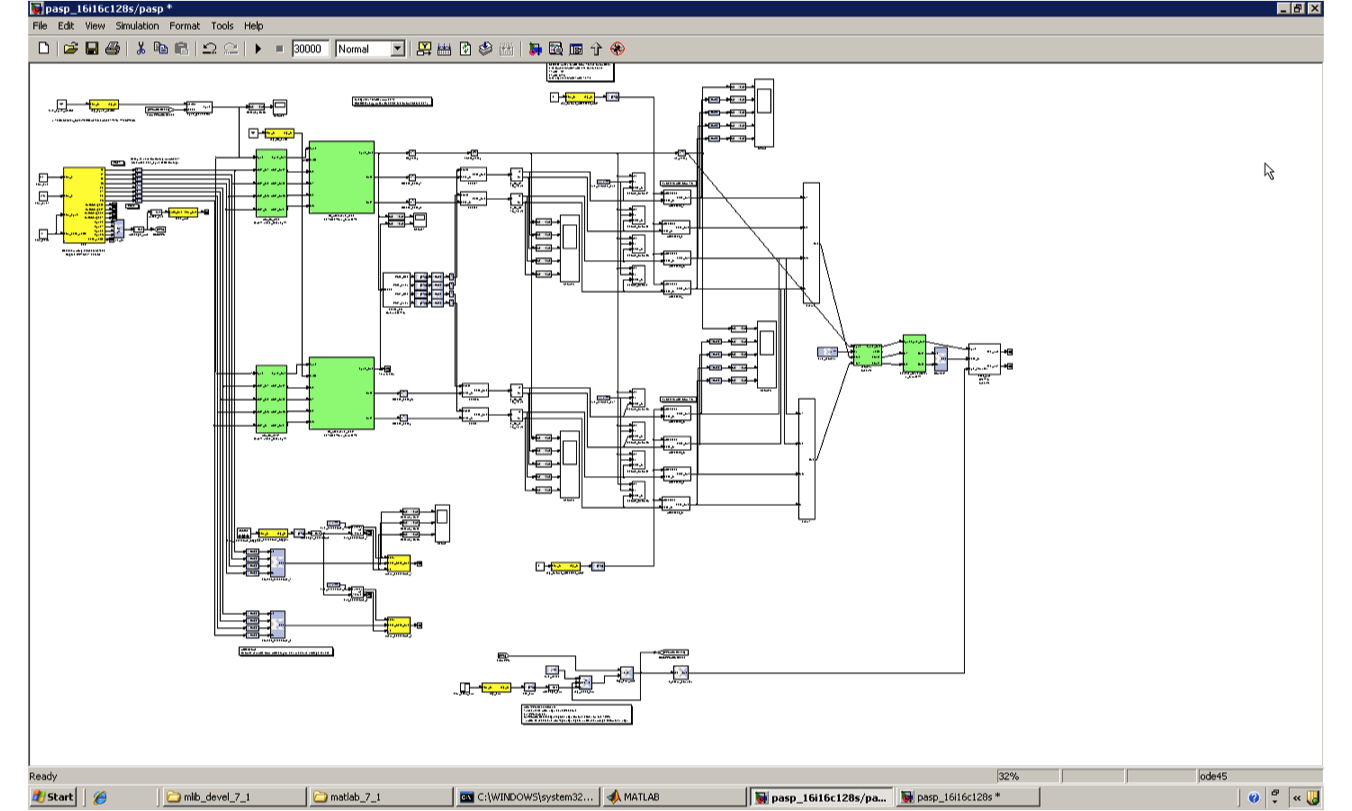
\includegraphics[width=1\textwidth]{Images/C4/pasp_low_level.png}
  \caption{TODO}
  \label{fig: C4/pasp_low_level.png}
\end{figure}

The instruments generated with this package use a heterogeneous design, allowing us to benefit from the strengths of FPGAs and GPUs. 
The FPGA board is able to sample and process very high bandwidths that a single CPU or GPU would not be able to manage; 
once the FPGA has split up the band the GPU provides a platform that is easier than an FPGA to program but still provides high compute power. 
A design called the Packetized Astronomy Signal Processor, or PASP, is run on the FPGA.
PASP splits up the large band into smaller bands that can be processed using off the shelf servers.
The subbands are put into packets on the FPGA and sent over a 10 gigabit Ethernet switch to a cluster of servers.
The servers receive the data from the switch and process it using spectroscopy software provided in the software package or special purpose application software written by the user and linked into the provided packet processing infrastructure.

Figure \ref{fig:spec_highlevel} shows a high level view of a spectrometer that could be designed with this package. 
In this example, a ROACH board divides the input band into 64 subbands and sends them out to a 16 server cluster.
An ADC is used to digitize data from the telescope and connects to the ROACH board via Z-DOK connectors. 
The digitized data is split into 64 subbands and sent through a 10 gigabit Ethernet switch.
Each server in the cluster receives and processes 4 subbands.

\begin{figure}[ht!]
  \centering
     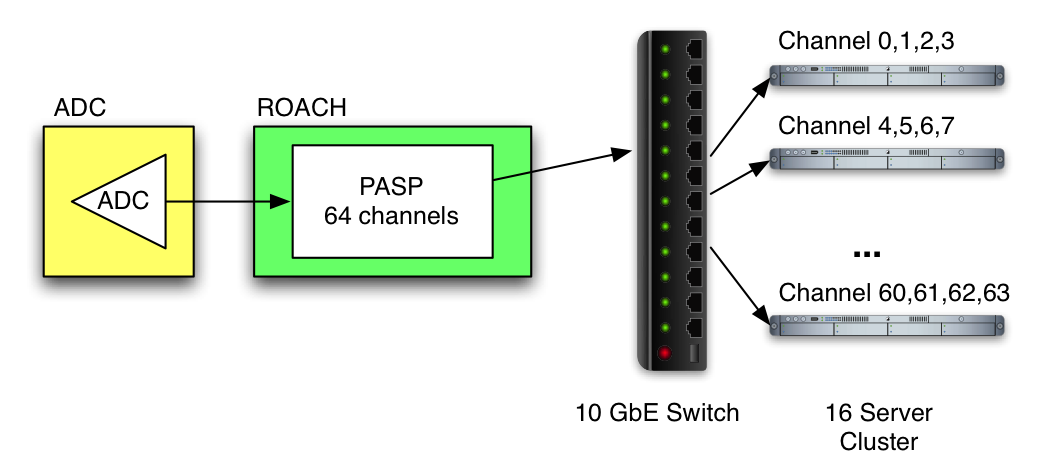
\includegraphics[width=1\textwidth]{Images/C4/spec_highlevel.png}
  \caption{Example high level instrument architecture}
  \label{fig:spec_highlevel}
\end{figure}

\subsubsection{Server Software}
Our package includes spectroscopy software that interfaces with the PASP design.
This software receives data over an Ethernet port and transfers it from the CPU to the GPU. 
The GPU runs an FFT and then sends the data back to the CPU to be recorded.
The GPU software, like the GPU benchmark, uses the CUFFT library to run FFT. 
The FFT size depends on the desired resolution for a specific application and an efficient batch size can be determined by running the FFT benchmark to find the best batch size for the given FFT size.

The server software was designed so other applications could easily be implemented on the GPU without altering or rewriting the receive code that interprets the packet headers and transfers data to the GPU.
Once the data is on the GPU, the software calls a process function and passes it a pointer to the GPU data.
An initialization function is called before the data processing begins to do any setup needed by the processing function, and an corresponding destroy function cleans up once the processing is complete.
In the spectroscopy software included in the package, the initialization function creates the FFT plan, the processing function calls CUFFT, and the destroy function deletes the FFT plan.
Modifying the application run on the GPU simply requires a redefinition of these three functions.
Using this interface, we successfully replaced the CUFFT processing with software developed for SETI searches designed by Kondo et al. \cite{Kondo:2010uk}.

In this paper, we describe a radio astronomy instrument that is easily reconfigured to suit a variety of applications.
%Figure \ref{fig: universal_arch} shows how this style of instrument design can be extended to a heterogeneous cluster running multiple processing algorithms at the same time.
All of these algorithms require the data to be broken up into subbands before it can be processed by the server which can be done on the same FPGA. 
Using multicast packets, multiple servers can subscribe to the same subbands generated on by PASP and process them in different ways. 


This style of instrument design greatly accelerates time to science for many projects.
Separating the implementation of the instrument from the hardware specification has created a design that works well for a variety of computational resources and applications.
As resources improve, the instrument can improve along with them, providing the opportunity to do new science that wasn't possible before.



